\documentclass[a4paper,11pt]{jsarticle}


% 数式
\usepackage{amsmath,amsfonts}
\usepackage{bm}
% 画像
\usepackage[dvipdfmx]{graphicx}
\usepackage{listings,jvlisting}
\usepackage{float}
\lstset{
  basicstyle={\ttfamily},
  identifierstyle={\small},
  commentstyle={\smallitshape},
  keywordstyle={\small\bfseries},
  ndkeywordstyle={\small},
  stringstyle={\small\ttfamily},
  frame={tb},
  breaklines=true,
  columns=[l]{fullflexible},
  numbers=left,
  xrightmargin=0zw,
  xleftmargin=3zw,
  numberstyle={\scriptsize},
  stepnumber=1,
  numbersep=1zw,
  lineskip=-0.5ex
}

\begin{document}

\title{画像実験課題3}
\author{1029323422 天野岳洋}
\date{\today}
\maketitle
\clearpage

\section{概要}
課題2からコードを改良し, パラメータを学習するプログラムを作成する.

\section{設計の方針}
基本的には課題2の内容に加え定義通り逆伝播層を導入し, 学習率に基づいて更新を行う.
それを何度か繰り返しを行えばよい.ただし,
伝播層と逆伝播層では行列の形が違うことに注意する.

\section{実装}
\subsection*{前準備}
三層NNで必要になる変数の準備を行う. 実装の具体的なコードは以下のとおりである.
\begin{lstlisting}[caption=前準備]
  import numpy as np
  import mnist

  seed, M, C, B = 601, 80, 10, 100
  #study_rate
  my = 0.01
  np.random.seed(seed)
  X = mnist.download_and_parse_mnist_file("train-images-idx3-ubyte.gz")
  Y = mnist.download_and_parse_mnist_file("train-labels-idx1-ubyte.gz")
  img_size = X[0].size
  epoch = X.shape[0] // B
  #epoch_repeat
  num = 30

  W1 = np.random.normal(loc = 0, scale = np.sqrt(1/img_size), size=(M, img_size))
  b1 = np.random.normal(loc = 0, scale = np.sqrt(1/img_size), size=(M, 1))
  W2 = np.random.normal(loc = 0, scale = np.sqrt(1/M), size=(C, M))
  b2 = np.random.normal(loc = 0, scale = np.sqrt(1/M), size=(C, 1))
\end{lstlisting}
\par
課題2以前で説明した内容については省略する.
新しく導入したものとして, my, epoch, numがある.
myは学習率であり, 教科書通り0.01としている.
epochは1epochで何回繰り返すかを表しており, データ数//バッチサイズ
によって求めている. numは何epoch繰り返すかを表しており, これは適当な数字を
用いている.

\subsection*{ロード}
パラメータの初期化方法として, ランダム初期化以外に, ロードによる
初期化も必要である. これを可能にするコードは以下のとおりである.
\begin{lstlisting}[caption = load]
  print("random -> 0, load -> 1")
  a = int(input())
  if(a == 1):
    parameters = np.load("./Parameters/parameter.npz")
    W1 = parameters['arr_0']
    W2 = parameters['arr_1']
    b1 = parameters['arr_2']
    b2 = parameters['arr_3']
\end{lstlisting}
内容については容易であるため, 省略する.

\subsection*{学習}
ここではまとめて三層NNのパラメータを更新する手続きについて説明を行う.
ただし, back-propagationについての説明は後のセクションで詳しく行う.
実装の具体的なコードは以下のとおりである.
\begin{lstlisting}[caption=3NN]
  for i in range(num):
    for j in range(epoch):
        batch_random = np.random.randint(0, 60000, B)       
        before_conv = np.array(X[batch_random])
        img = before_conv.reshape((B, img_size, 1))
        answer = np.array(Y[batch_random])
        #one-hot vectorize
        onehot = np.zeros((answer.size, 10))
        onehot[np.arange(answer.size), answer] = 1
        onehot = onehot.reshape(B, C, 1)
        

        #propagation
        input1 = np.matmul(W1, img) + b1
        output1 = 1/(1 + np.exp(-1 * input1))
        input2 = np.matmul(W2, output1) + b2
        alpha = np.repeat(input2.max(axis = 1), C, axis= 1).reshape(B, C, 1)
        sumexp = np.repeat(np.sum(np.exp(input2 - alpha), axis=1), 10, axis=1).reshape(B, C, 1)
        output_last = np.exp(input2 - alpha) / sumexp
        crossE += (-1/B)* np.sum(onehot * np.log(output_last))

        #back
        delta_b = ((output_last - onehot)/B).reshape(B, C).T

        delta_y1 = np.dot(W2.T, delta_b)
        delta_W2 = np.dot(delta_b, output1.reshape(B, M))
        delta_b2 = np.sum(delta_b, axis = 1).reshape(C, 1)

        delta_a = delta_y1 * (1 - output1.reshape(B, M).T) * output1.reshape(B, M).T

        delta_x = np.matmul(W1.T, delta_a)
        delta_W1 = np.matmul(delta_a, img.reshape(B, img_size))
        delta_b1 = np.sum(delta_a, axis=1).reshape(M, 1)

        #update
        W1 = W1 - my * delta_W1
        b1 = b1 - my * delta_b1
        W2 = W2 - my * delta_W2
        b2 = b2 - my * delta_b2
    print(crossE / epoch)
  print("finish")
  np.savez("parameter", W1, W2, b1, b2)
\end{lstlisting}
まず初めに説明した数だけの繰り返しを行っている.
その後, 課題2でやった通りの方法で, 画像の適切な形への変更,
one-hotvecorの作成, 順伝播を行っている. そして微分を計算して,
それに学習率をかけた分だけそれぞれのパラメータから引いている.
\par
後処理としては, 1epochが終わるたびにcrossEntropyを出力, すべてのepoch
が終われば, finishという文字列を出力し, パラメータをparameterというファイルに保存している.

\subsection*{逆伝播層}
ここでは, 逆伝播層についての詳しい説明を行う.
\subsubsection*{ソフトマックス層}
まずは形を確認する.ソフトマックス層に置ける入力の形は
(B, C, 1), 出力の形も同じく(B, C, 1)である. したがって, 入力についての偏微分は,
$y_{ik1}^{(2)}$を3NNのバッチ内のi番目の画像に対する数字kに関する最終的な出力, $y_{ik1}$をonehot\_vectorのバッチ内i番目の数字kに
関する値であるとすると,
$$\frac{\partial E_n}{\partial a_{ik1}} = \frac{y_{ik1}^{(2)} - y_{ik1}}{B}$$
によって求められ, この左辺の形は(B, C, 1)である.
\par
ここでは次の全結合層で求められる形が(C, B)であることから,
あらかじめその形に変形しておく.その説明は次のセクションで行う.
以上の手続きを行うコードは以下のとおりである.
\begin{lstlisting}[caption=SoftMax]
  delta_b = ((output_last - onehot)/B).reshape(B, C).T
\end{lstlisting}

\subsubsection*{全結合層}
全結合層においては, 出力の偏微分が与えられており, それに基づいて,
入力, 重み, バイアスについての偏微分を行うものとする. この理由として,
全結合層が最後の出力層となることは考えにくいので, 一つ出力層に近い層の
入力に関する微分値が与えられているはずだからである.\par
では詳しい計算の手続きを述べる.
出力の偏微分は,$\bm{y_i}$をミニバッチ内i番目の出力
(=後ろの層の入力)
であるとし、$\partial E_N / \partial \bm{y_i}$を各列に持つ行列を
$\partial E_N / \partial Y$として与えられているものとする.
つまり, $\partial E_N / \partial Y$は(?, B)という形をしているものである.
?に入る数字は二つ目の全結合層であるならば, Cであり, 一つ目の
全結合層ならば, Mである. この形に注意を払えば後は教科書通りであり,

\begin{gather}
  \frac{\partial E_n}{\partial X} = W^T \frac{\partial E_n}{\partial Y} \\
  \frac{\partial E_n}{\partial W} = \frac{\partial E_n}{\partial Y} X^T \\
  \frac{\partial E_n}{\partial \bm{b}} = rowSum (\frac{\partial E_n}{\partial Y} X^T)
\end{gather}
によって, それぞれの微分値が求められる.ただし,
$\partial E_n / \partial X$の行列の形は入力(B, X, 1)とは異なり,
(X, B)という形になっていることに注意したい.
実際のコードは以下の通りである.
\begin{lstlisting}[caption = 全結合層2]
  delta_y1 = np.dot(W2.T, delta_b)
  delta_W2 = np.dot(delta_b, output1.reshape(B, M))
  delta_b2 = np.sum(delta_b, axis = 1).reshape(C, 1)
\end{lstlisting}
\par
ここでは, 伝播層では入力を(B, M, 1)として与えていたものを,
(B, M)に変更しているほか, delta\_b2の形を引き算ができるように,
(C, )から(C, 1)へと変更している. また, delta\_bは前の節で得たものであり,
適切な形へと変更されている.もう一つの全結合層については説明を省略する.
実際のコードは以下のとおりである.
\begin{lstlisting}[caption = 全結合層1]
  delta_x = np.matmul(W1.T, delta_a)
  delta_W1 = np.matmul(delta_a, img.reshape(B, img_size))
  delta_b1 = np.sum(delta_a, axis=1).reshape(M, 1)
\end{lstlisting}

\subsubsection*{シグモイド関数}
シグモイド関数への入力を$x_{ik1}$とし, 出力を$y_{ik1}$として,
$ \partial E_n / \partial y_{ki}$が与えられたときに,
$$ \frac{\partial E_n}{\partial x_{ki}} =
  \frac{\partial y_{ki}}{\partial x_{ki}} \frac{\partial E_n}{\partial y_{ki}}=
  \frac{\partial E_n}{\partial y_{ki}} (1 - y_{ki}) y_{ki}
$$

これを実行するコードは以下のとおりである.
\begin{lstlisting}[caption=シグモイド関数]
  delta_a = delta_y1 * (1-output1.reshape(B, M).T) * output1.reshape(B, M).T
\end{lstlisting}

\section{実際の動作}
実際に実行すると以下のような標準出力が得られた.
\begin{lstlisting}
  2.1195802822692515
  1.6942129635495269
  1.2908205032287965
  1.0160632470686923
  0.8537015611381444
  ...
\end{lstlisting}
さらに, parameter.npzというファイルが保存されていることを確認した.
\subsection{学習の様子}
学習の様子をテストデータ, トレーニングデータそれぞれに対しての正解率, 又はクロスエントロピー誤差
について注目することによって調べた. まず初めに少ないエポック数のグラフを乗せる.
\begin{figure}[H]
  \begin{tabular}{cc}
    \begin{minipage}[h]{0.45\linewidth}
      \centering
      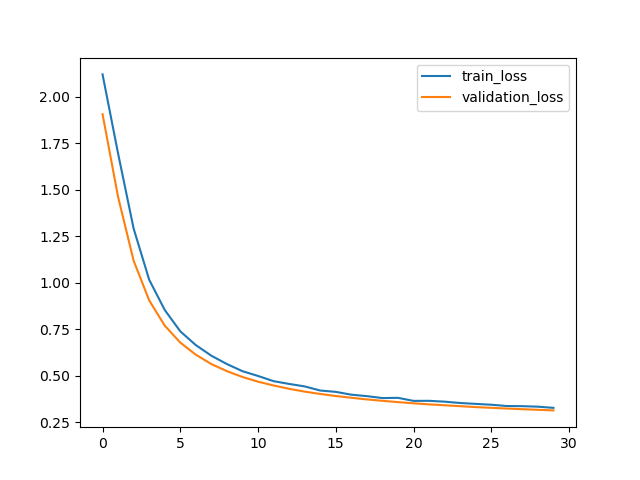
\includegraphics[keepaspectratio, scale = 0.4]{loss.png}
      \caption{mini\_loss}
    \end{minipage} &

    \begin{minipage}[h]{0.45\linewidth}
      \centering
      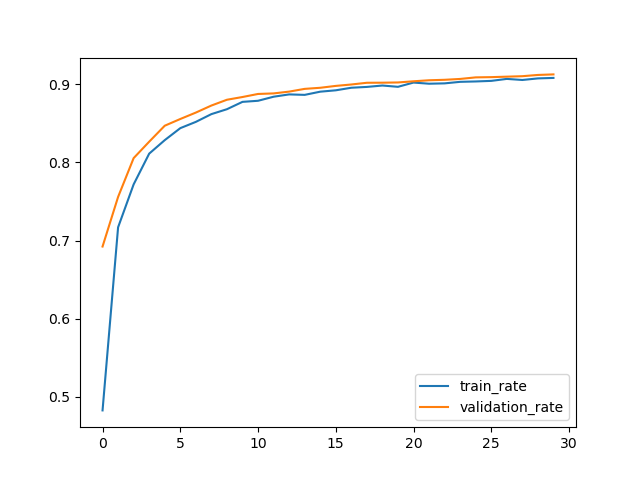
\includegraphics[keepaspectratio, scale = 0.4]{rate.png}
      \caption{mini\_rate}
    \end{minipage}
  \end{tabular}
\end{figure}

このグラフを見れば, うまく学習が進んでいることがわかる. テストデータに対しての方が
成績が良くなっているのは, 訓練データに対して学習させたのちに, テストデータに対して
パフォーマンスを図っているためである. この次にエポック数を10000にして収束を図る.
それが次のグラフである.

\begin{figure}[H]
  \begin{tabular}{cc}
    \begin{minipage}[h]{0.45\linewidth}
      \centering
      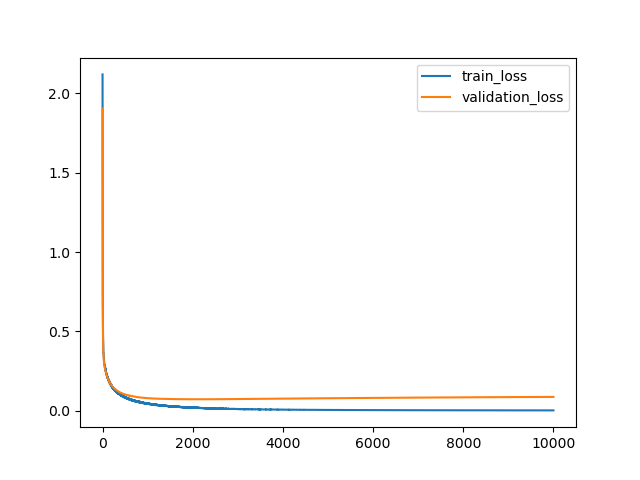
\includegraphics[keepaspectratio, scale = 0.4]{overfitting_loss.png}
      \caption{mini\_loss}
    \end{minipage} &

    \begin{minipage}[h]{0.45\linewidth}
      \centering
      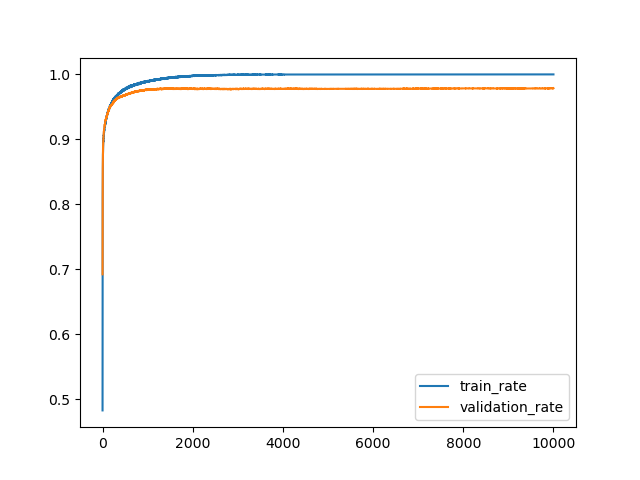
\includegraphics[keepaspectratio, scale = 0.4]{overfitting_rate.png}
      \caption{mini\_rate}
    \end{minipage}
  \end{tabular}
\end{figure}

上の二つのグラフを見れば, 最終的に訓練データに対しての正答率は100\%に限りなく近い
値になっていることがわかる. またその際のクロスエントロピー誤差は0.0016となった.
一方でテストデータに対しての正答率は0.95\%を目安にとどまった. 

\end{document}